\documentclass[./\jobname.tex]{subfiles}
\begin{document}
\chapter {Experiment 1: Parallel Population JADE}
\label{chap:experimet_1}

With the serial algorithm from the chapter above, evaluating a \gls{pde} takes way to long to be practically relevant (beyond $14.5 \cdot 10^3$ seconds at $10^6$ \gls{nfe}). To reduce the solving time and speed up all further experiments, a parallel JADE is implemented. This chapter describes the benefits and drawbacks of the new algorithm.  

\section{Hypotheses}
The actual parallel JADE algorithm is shown in appendix \ref{chap:pseudocode_pjade}. The pseudocode \ref{algo: pjade} is very similar to the JADE algorithm \ref{algo: jade}. The main differences are laid out in the code-lines 11 to 17. The mutation, the crossover, the parameter adaption and the fitness evaluation are done in parallel for each individual in the population. The parallelism is based on the python module multiprocessing (\cite{python_standard_library_multiprocessing_2020}), in particular the \inlinecode{multiprocessing.Pool.apply\_async(func, *args)} method. This method takes a function, in this case an adapted version of the for-loop from code-line 11 to 17, and automatically maps it to a number of preallocated processes. After this is done for every individual in the population, the processes are synchronised and the results get returned to the main process. Therein lies the actual difference to the serial JADE. In the parallel algorithm new individuals are only available after each generation, whereas with the serial algorithm, the individuals are constantly updated before the next generation starts. This means that in the parallel algorithm information is withheld until the next generation - the same information can spread faster in the serial algorithm.  

For the sake of completeness, the memetic parallel JADE pseudocode is shown in the algorithm \ref{algo: memeticpJADE} below. The only difference compared to the simple memetic JADE \ref{algo: memeticJADE} is the usage of the pJADE in code-line 5. 

\begin{algorithm}[h]
	\SetAlgoNoLine
	\DontPrintSemicolon
	\SetKwFunction{FmpJADE}{memeticpJADE}
	\SetKwProg{Fn}{Function}{:}{}
	\Fn{\FmJADE{$\mathbf{X}$, $funct$, $minErr$, $maxFE$}}{
		$dim$, $popsize$ $\gets size(\mathbf{X})$\;
		$p \gets 0.3$\;
		$c \gets 0.5$\;
		$pop$, $FE$, $F$, $CR$ $\gets pJADE($$\mathbf{X}$, $p$, $c$, $funct$, $minErr$, $maxFE - 2 dim$ $)$\;
		$bestIndex = argmin(FE)$\;
		$bestSol = pop[bestIndex]$\;
		$pop$, $FE$ $ = downhill\text{ }simplex($$funct$, $bestSol$, $minErr$, $2 dim)$\;
		\Return $pop$, $FE$, $F$, $CR$
	}
	\unterschrift{Pseudocode of memetic parallel JADE}{}{}
	\label{algo: memeticpJADE}
\end{algorithm}

This chapter discusses the question if the explained distinctions actually influence the results, to the better or the worse. Further, the time-benefits of this strategy are examined and assessed.

\section{Experiment Setup}
Similar to the experiment 0 before, the standard parameters from table \ref{tab:ci_parameter} are used. Again, two different machines with either $10^4$ \gls{nfe} ($\rightarrow$ machine 1) or $10^6$ \gls{nfe} ($\rightarrow$ machine 2) are used, whereby the time comparison is only allowed on machine 1. Also, 5 \gls{gak} are used, meaning the problem dimension is 20 and the population size is 40. The standard Wilcoxon test (explained in appendix \ref{chap:apendix_post_proc}) is used to proof statistical significance. 

Additionally, a new parameter is introduced: the number of allocated parallel processes. Typically, this parameter is set to the number of available processors, but this also depends on the general workload of the machine. When using too many processes, the system might be overwhelmed, effectively slowing down the task and resulting in an even longer solving time. On machine 1, 5 processes are implemented, while machine 2 is capable of handling 30 processes. With other machines, it might be possible to introduce even more processes, potentially increasing the speed-up even further. 

\section{Results}

The two images \ref{fig:parallel_jade_time_boxplot} and \ref{fig:parallel_jade_memory_boxplot} display a boxplot of the time- and memory usage. To ensure comparability with the results obtained for the serial JADE, these images represent the results at $10^4$ \gls{nfe} on machine 1. 

\begin{figure}[H]
	\centering
	\noindent\adjustbox{max width=0.66\linewidth}{
		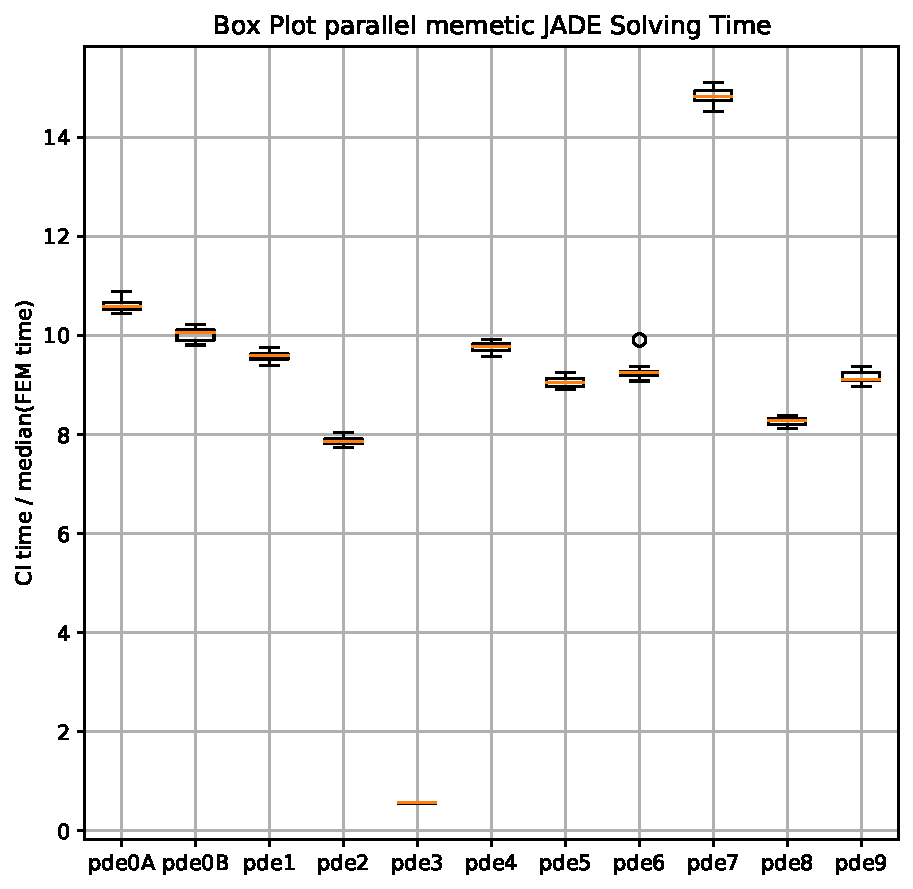
\includegraphics[width=\textwidth]{../../code/experiments/experiment_1/time_boxplot_ci_exp1.pdf}
	}
	\unterschrift{Relative solving time results of parallel memetic JADE after $10^4$ \gls{nfe}.}{}{}
	\label{fig:parallel_jade_time_boxplot}
\end{figure}


\begin{figure}[H]
	\centering
	\noindent\adjustbox{max width=0.66\linewidth}{
		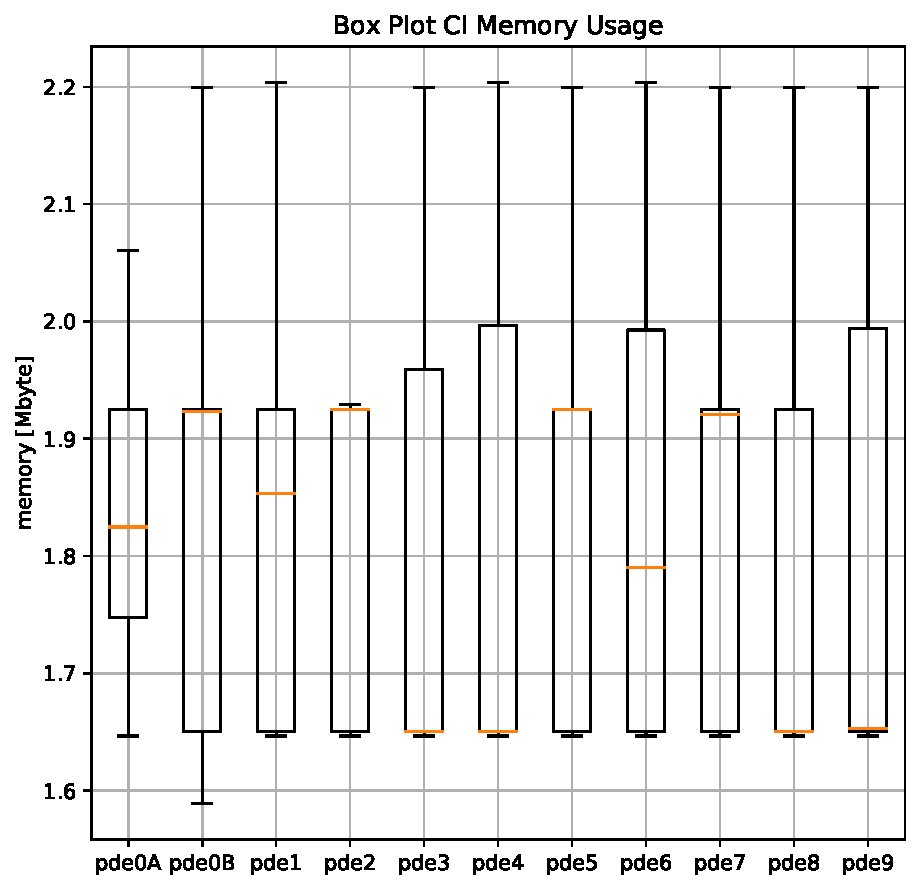
\includegraphics[width=\textwidth]{../../code/experiments/experiment_1/mem_boxplot_ci_exp1.pdf}
	}
	\unterschrift{Relative memory usage results of parallel memetic JADE after $10^4$ \gls{nfe}.}{}{}
	\label{fig:parallel_jade_memory_boxplot}
\end{figure}



Table \ref{tab:compare_parallel_serial_jade_10^6} shows the mean and the median L2 norm reached on the testbed by both the serial and the parallel algorithm. This is completed with a Wilcoxon test, to identify the difference in the performance. The term ``undecided'' in this context means that the mean and the median paint different pictures: one of those values is smaller while the other one is larger. Most notably, on \gls{pde} 4 the parallel JADE performs significantly worse than the serial JADE. 

\begin{table}[H]
	\centering
	\noindent\adjustbox{max width=\linewidth}{
		\begin{tabular}{|c|c|c|c|c|l|}
			
			\hline
			\rowcolor[HTML]{\farbeTabA}
			
			Algorithm & \multicolumn{2}{|c|}{serial JADE} & \multicolumn{2}{|c|}{parallel JADE} & \\ \hline
			stat & mean & median & mean & median & Wilcoxon Test \\ \hline \hline
			\gls{pde} 0A & 0.6596 $\pm$ 0.5510 & 0.9285 & 0.6939 $\pm$ 0.6635 & 0.9243 & unsig. undecided \\ \hline
			\gls{pde} 0B & 0.2027 $\pm$ 0.1302 & 0.1516 & 0.2809 $\pm$ 0.3071 & 0.2035 & unsig. worse \\ \hline
			\gls{pde} 1 & 0.0149 $\pm$ 0.0049 & 0.0151 & 0.0239 $\pm$ 0.0467 & 0.0146 & unsig. undecided \\ \hline
			\gls{pde} 2 & 0.0257 $\pm$ 0.0140 & 0.0224 & 0.0300 $\pm$ 0.0157 & 0.0255 & unsig. worse \\ \hline
			\gls{pde} 3 & 0.0328 $\pm$ 0.0169 & 0.0285 & 0.0371 $\pm$ 0.0206 & 0.0295 & unsig. worse \\ \hline
			\gls{pde} 4 & 0.0378 $\pm$ 0.0083 & 0.0352 & 0.0505 $\pm$ 0.0121 & 0.0481 & sig. worse \\ \hline
			\gls{pde} 5 & 1.1968 $\pm$ 0.0286 & 1.2056 & 1.2030 $\pm$ 0.0465 & 1.2053 & unsig. undecided \\ \hline
			\gls{pde} 6 & 0.4135 $\pm$ 1.2133 & 0.0018 & 0.5814 $\pm$ 1.3550 & 1.266E-17 & unsig. undecided \\ \hline
			\gls{pde} 7 & 0.0221 $\pm$ 0.0019 & 0.0223 & 0.0228 $\pm$ 0.0025 & 0.0226 & unsig. worse \\ \hline
			\gls{pde} 8 & 0.2170 $\pm$ 0.0019 & 0.2175 & 0.2167 $\pm$ 0.0017 & 0.2169 & unsig. better \\ \hline
			\gls{pde} 9 & 0.0451 $\pm$ 0.0119 & 0.0459 & 0.0426 $\pm$ 0.0115 & 0.0463 & unsig. undecided \\ \hline
			
		\end{tabular}
	}
	\unterschrift{This table compares the results obtained by the parallel and the serial JADE. All results are obtained at $10^6$ \gls{nfe}. The serial data is the same as already presented in table \ref{tab:serial_jade_compare_10^6_10^4}. }{}{}
	\label{tab:compare_parallel_serial_jade_10^6}
\end{table}



\section{Discussion}

The results from above are analysed in this chapter. The time and memory usage as well as the speed-up for every testbed function is discussed. Further, the significant worse results on \gls{pde} 4 are investigated. Finally, the usage of the parallel JADE in all further experiments is justified. 

\subsection{Memory Usage}
As the boxplot \ref{fig:parallel_jade_memory_boxplot} shows, the memory usage is roughly at the same level, somewhere between 1.5 to 4.0 percent of \gls{fem} solver. The memory usage is very similar to the serial experiment. This is expected, since memory-wise no integral changes have been performed.  

\subsection{Solving Time}
The main purpose of the parallelisation is to cut down the solving time and accelerate all further experiments. To that extent, the population is evaluated in parallel. As the solving time boxplot in figure \ref{fig:parallel_jade_time_boxplot} shows, this goal was achieved. The execution time after $10^4$ \gls{nfe} now ranks between the 8 and 15-fold of the \gls{fem} solver. This is unquestionably faster than the solving time of the serial algorithm. Remarkable is that on \gls{pde} 3, the \gls{ci} solver is even faster than NGSolve and takes only about $0.56 \cdot 65.2 \text{ s} \approx 36.5 \text{ s}$. Of course, to compete with the solution quality, more \gls{nfe} are needed, which increases the execution time. 

Image \ref{fig:serial_to_parallel_speedup} shows the calculated mean \gls{sp} over 20 replications, that is accomplished by substituting the serial JADE with the parallel version. The 95\% confidence interval is shown in yellow. 

\begin{figure}[H]
	\centering
	\noindent\adjustbox{max width=0.8\linewidth}{
		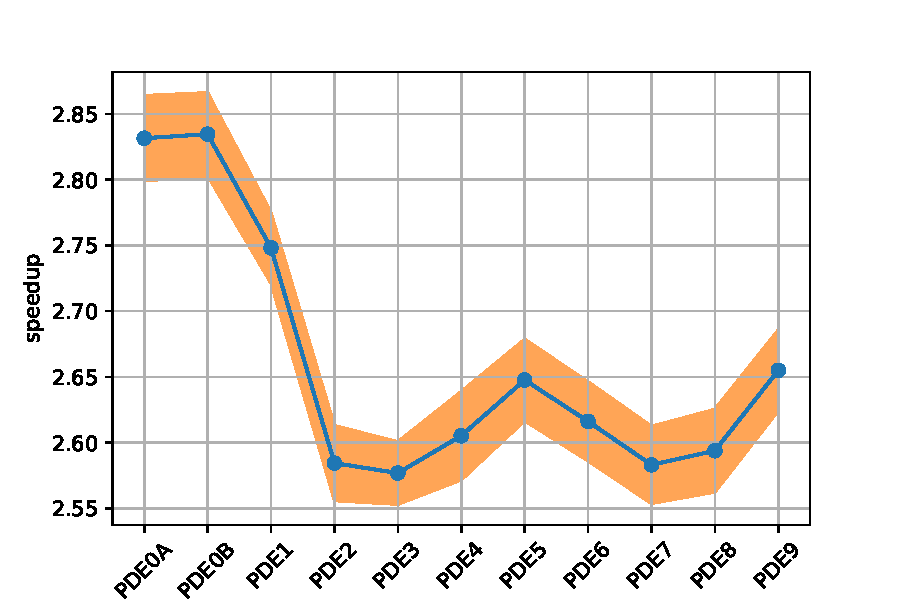
\includegraphics[width=\textwidth]{../../code/experiments/experiment_1/speedup_plot.pdf}
	}
	\unterschrift{Mean speed-up of parallel JADE with 95\% confidence interval.}{}{}
	\label{fig:serial_to_parallel_speedup}
\end{figure}

The plot \ref{fig:serial_to_parallel_speedup} shows that the speed-up varies by testbed function. This can be directly linked to the ``size'' of the fitness function, especially the \gls{rhs} of the \gls{pde}. The longer the fitness function takes to evaluate, the greater is the speed-up that can be achieved ($time(fit \text{ } evaln) \uparrow \rightarrow sp \uparrow$). One would expect the same correlation for the size of the population: the larger a population, the better is the speed-up ($pop \text{ } size \uparrow \rightarrow sp \uparrow$). Larger fitness functions are needed by the testbed \gls{pde}s 0A, 0B, 1, 5, and 9. Looking at the definition of these equations in appendix \ref{chap:testbed}, it is notable that the \gls{rhs} are constructed of more terms compared to the other equations. 

\subsection{PDE 4}

Table \ref{tab:compare_parallel_serial_jade_10^6} shows that the L2 norm achieved on \gls{pde} 4 is significantly worse when the parallel JADE is used. This is not expected and hinders the justification of substituting the serial JADE with the parallel version. It is of interest to confirm the hypothesis and allow the usage of the parallel JADE in all further experiments. 

The absolute error (calculated by $E_{abs} = \left| u_{apx}(x_0, x_1) - u_{ext}(x_0, x_1) \right|$) of the worst solution generated either by the serial or the parallel algorithm can be seen in the plot from figure \ref{fig:serial_parallel_pde4_error_comparison}. The plot suggests that the underlying structure of the error is similar in both cases. Although, the L2 norm, the fitness value and the \gls{rmse} are lower with the serial JADE, the absolute error values from the plot are similar. Only on the boundary $x_1 = 0, x_0 \in [0,1]$, the serial JADE generates a visually smaller error. 

\begin{figure}[H]
	\centering
	\begin{subfigure}[b]{0.5\linewidth}
		\centering
		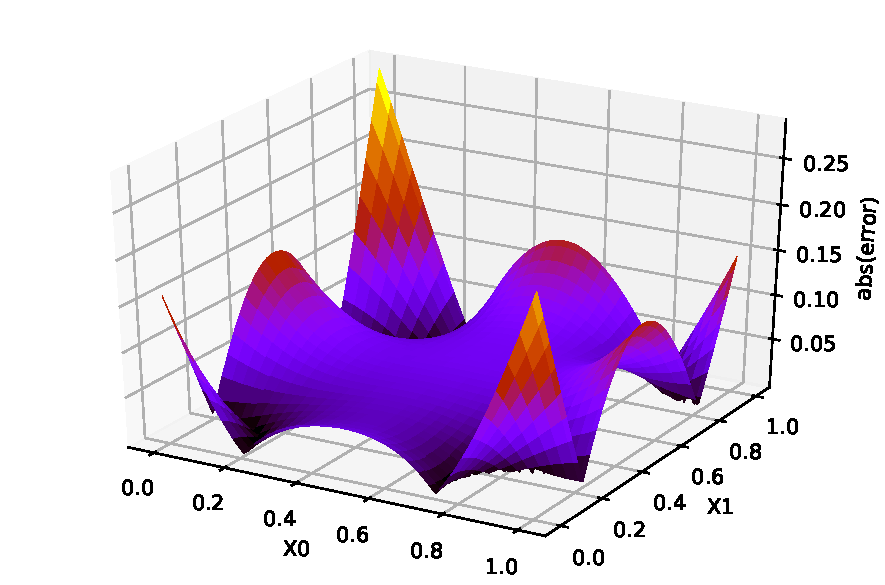
\includegraphics[width=1\textwidth]{../../code/experiments/experiment_1/abs_error_pde4_serial.pdf}
		\caption{Absolute error, serial JADE \\ L2 norm: 0.0608 \\ FE value: 0.4632 \\ RMSE: 0.0752}
		\label{fig:serial_JADE_pde4_abs_error}
	\end{subfigure}% 
	%
	\begin{subfigure}[b]{0.5\linewidth}
		\centering
		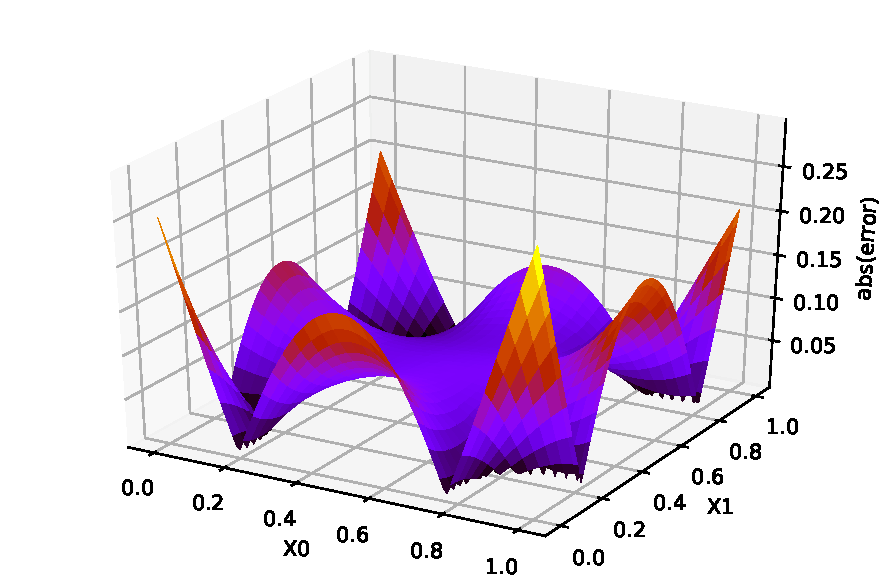
\includegraphics[width=1\textwidth]{../../code/experiments/experiment_1/abs_error_pde4_parallel.pdf}
		\caption{Absolute error, parallel JADE \\ L2 norm: 0.0733 \\ FE value: 0.6976 \\ RMSE: 0.0895}
		\label{fig:parallel_JADE_pde4_abs_error}
	\end{subfigure}%
	\unterschrift{Comparison of the absolute error of the worst solution on \gls{pde} 4 by a parallel and a serial memetic JADE at $10^6$ \gls{nfe}}{}{}%
	\label{fig:serial_parallel_pde4_error_comparison}
\end{figure}


In order to make the results easier to interpret, the histogram from figure \ref{fig:pde4_ex0_ex1_histogram} shows the L2 norm data from table \ref{tab:compare_parallel_serial_jade_10^6}. The best solutions of both algorithms are at a similar quality level. The parallel sample introduces more results with a worse quality. The absolute numerical range of the quality is visualised in the boxplot \ref{fig:pde4_ex0_ex1_boxplot}. The Wilcoxon test asserts that the two shown distributions are significantly different. While this can be confirmed visually, it can also be seen that the differences are only marginal. 


\begin{figure}[H]
	\centering
	\noindent\adjustbox{max width=0.8\linewidth}{
		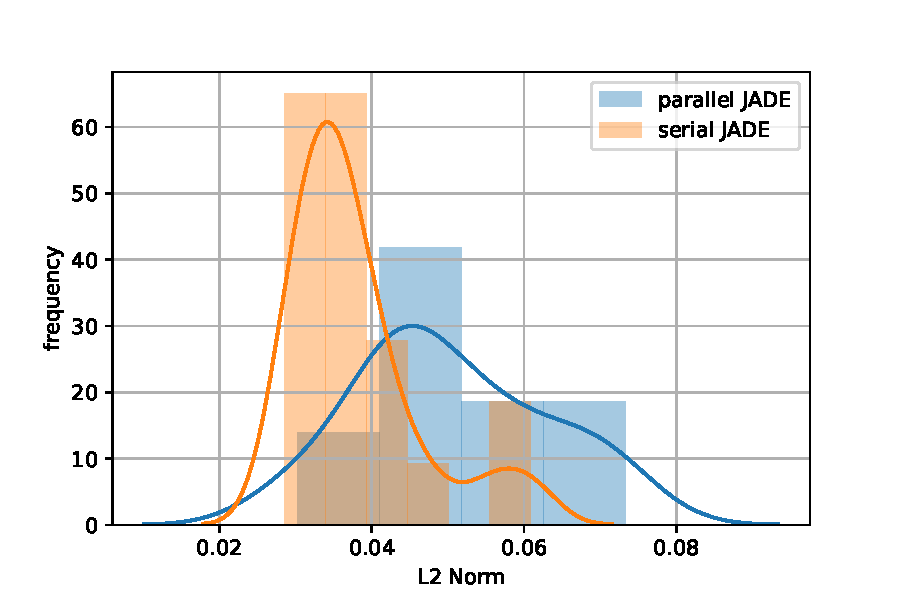
\includegraphics[width=\textwidth]{../../code/experiments/experiment_1/pde4_ex0_ex1_histogram.pdf}
	}
	\unterschrift{Histogram of the L2 norm data obtained by the serial and the parallel JADE on \gls{pde} 4 from table \ref{tab:compare_parallel_serial_jade_10^6}.}{}{}
	\label{fig:pde4_ex0_ex1_histogram}
\end{figure}

\begin{figure}[H]
	\centering
	\noindent\adjustbox{max width=0.52\linewidth}{
		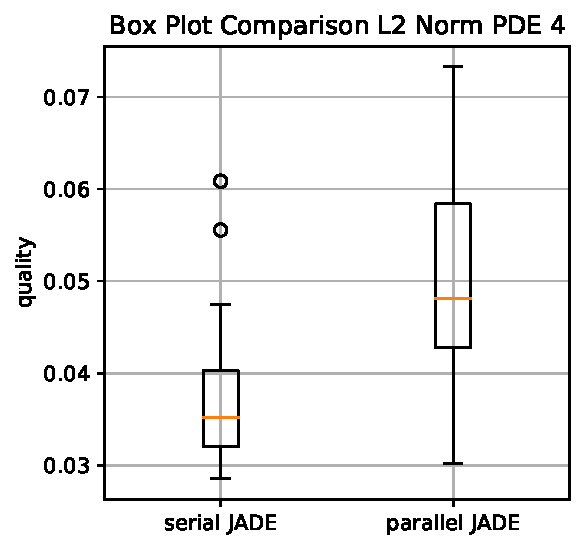
\includegraphics[width=\textwidth]{../../code/experiments/experiment_1/pde4_ex0_ex1_boxplot.pdf}
	}
	\unterschrift{Boxplot of the L2 norm data from table \ref{tab:compare_parallel_serial_jade_10^6} on \gls{pde} 4.}{}{}
	\label{fig:pde4_ex0_ex1_boxplot}
\end{figure}

Increasing the number of independent replications could provide further clues to that matter. Considering that quality-wise the parallel JADE makes no significant difference on 10 of 11 tested \gls{pde}s and the compelling speed-up on all test problems, the parallel JADE is applied in all further experiments. At the very worst, the algorithm is faster by a factor of 2.5 and results in a minor decrease of the solution quality. This trade-off is acceptable.


\end{document}